\documentclass[a4paper]{article}

\usepackage{amsmath,amsfonts,amsthm,amssymb}
\usepackage{graphicx}
\usepackage{physics}

\usepackage[]{mathpazo}
\usepackage{domitian}
\usepackage[T1]{fontenc}
\let\oldstylenums\oldstyle{}
\renewcommand{\baselinestretch}{1.5}

\author{}
\date{}

\begin{document}
\begin{center}
\bf \large Second Order Differential Equations Tutorial
\end{center}

{\bf \large Problem 8.}\\
{\bf \large Solution.}

The damped vibrating has equation
\begin{equation}
    m\ddot y+\lambda\dot y+ky=0
\end{equation}
with \(m=1\), \(k=25\) and \(\lambda=10\). It has the characteristic equation
\begin{equation}
    s^2+10s+25=0
\end{equation}
with characteristic root
\begin{equation}
    s=-5
\end{equation}

The solution is in the form of
\begin{equation}
    \boxed{y(t)=e^{-5t}(c_1+c_2t)}
\end{equation}
with initial conditions \(y(0)=0\) and \(\dot y(0)=0\).

The initial conditions are satisfied when \(c_1=1\) and \(c_2=5\).
\begin{equation}
    y(t)=e^{-5t}(1+5t)
\end{equation}
\begin{figure}[ht]
    \centering
    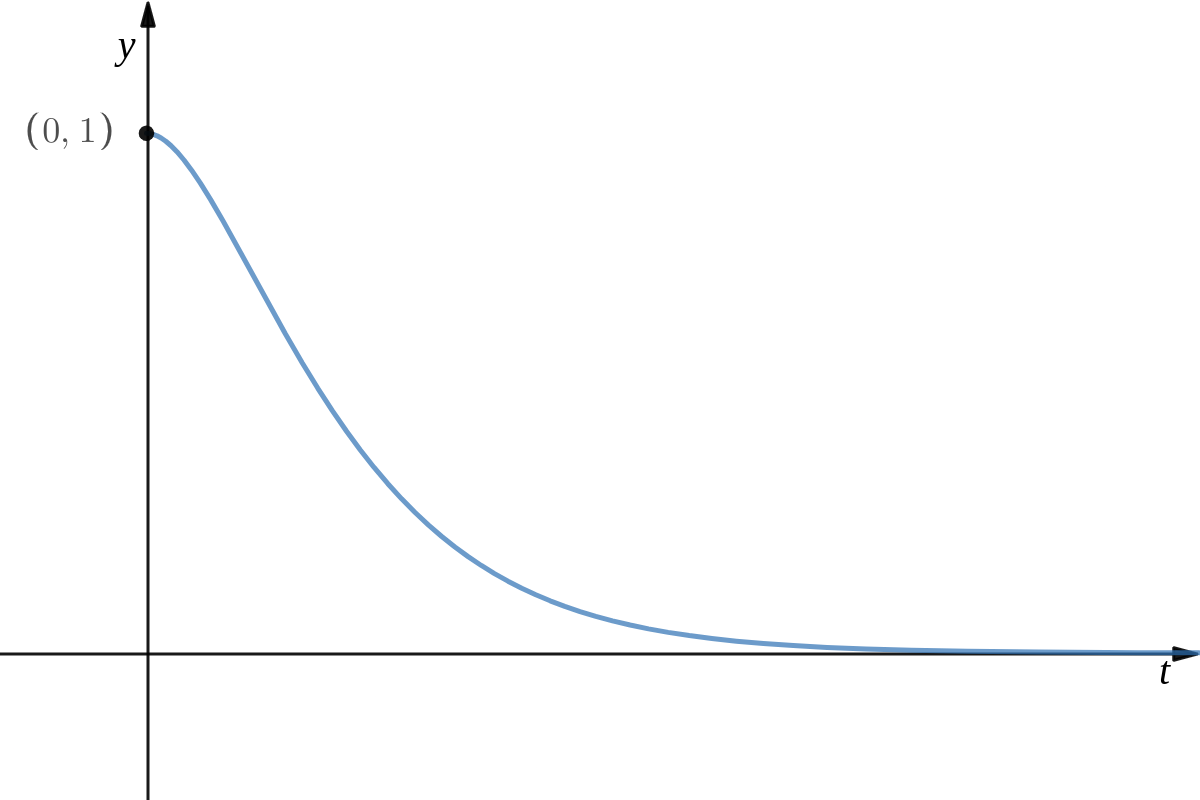
\includegraphics[width=0.69\textwidth]{so8.png}
    \caption{Graph of the equation of motion.}
\end{figure}

This motion is suitable to be used to close a door
because the door slows down as it approaches the door.

{\bf \large Problem 9.}\\
{\bf \large Solution.}

The tip of the tuning fork has equation
\begin{equation}
    m\ddot x+k\dot x+m\omega^2x=0
\end{equation}
with \(m>0\), \(k>0\), \(\omega>0\) and \(k^2\approx0\). It has the characteristic equation
\begin{equation}
    ms^2+ks+m\omega^2=0
\end{equation}
with characteristic root
\begin{equation}
    s=\frac{-k\pm\sqrt{k^2-4m^2\omega^2}}{2m}
    \approx\frac{-k\pm\sqrt{-{(2m\omega)}^2}}{2m}
    =-\frac k{2m}\pm i\omega
\end{equation}

The solution is in the form of
\begin{equation}
    x(t)=e^{-\frac k{2m}t}\left(c_1\cos(\omega t)+c_2\sin(\omega t)\right)
\end{equation}
with initial conditions \(x(0)=0\) and \(\dot x(0)=v\).

The initial conditions are satisfied when \(c_1=0\) and \(c_2=\frac v\omega\).
\begin{equation}
    \boxed{x(t)=\frac v\omega e^{-\frac k{2m}t}\sin(\omega t)}
\end{equation}

The period of the vibrations over time is constant, given by
\begin{equation}
    \Delta t=\frac{2\pi}\omega
\end{equation}

Let the time at the \(n^\text{th}\) time 
when the vibrations is at their maximum displacement be \(t_n\). 
The time at the first amplitude is
\begin{equation}
    t_1=\frac\pi{2\omega}
\end{equation}
which follows
\begin{equation}
    t_n=t_1+n\Delta t=\frac\pi{2\omega}+n\frac{2\pi}\omega
\end{equation}

Let the \(n^\text{th}\) amplitude of successive vibrations be \(A_n\), such that
\begin{equation}
    A_n=\frac v\omega e^{-\frac k{2m}t_n}
    =\frac v\omega e^{-\frac k{2m}\left(\frac\pi{2\omega}+n\frac{2\pi}\omega\right)}
    =\frac v\omega e^{-\frac{k\pi}{4m\omega}}\left(e^{-\frac{k\pi}{m\omega}}\right)^n
\end{equation}
Since \(A_n\) is in the form of \(ar^n\), it follows a geometric progression.

When \(k^2>4m^2\omega^2\), \(k^2-4m^2\omega^2>0\).
This means that the characteristic roots are real and distinct,
resulting in an overdamping case. In this case, \(x\) approaches 0 slowly as
time progresses, having a horizontal asymptote of \(x=0\).

\begin{figure}[ht]
    \centering
    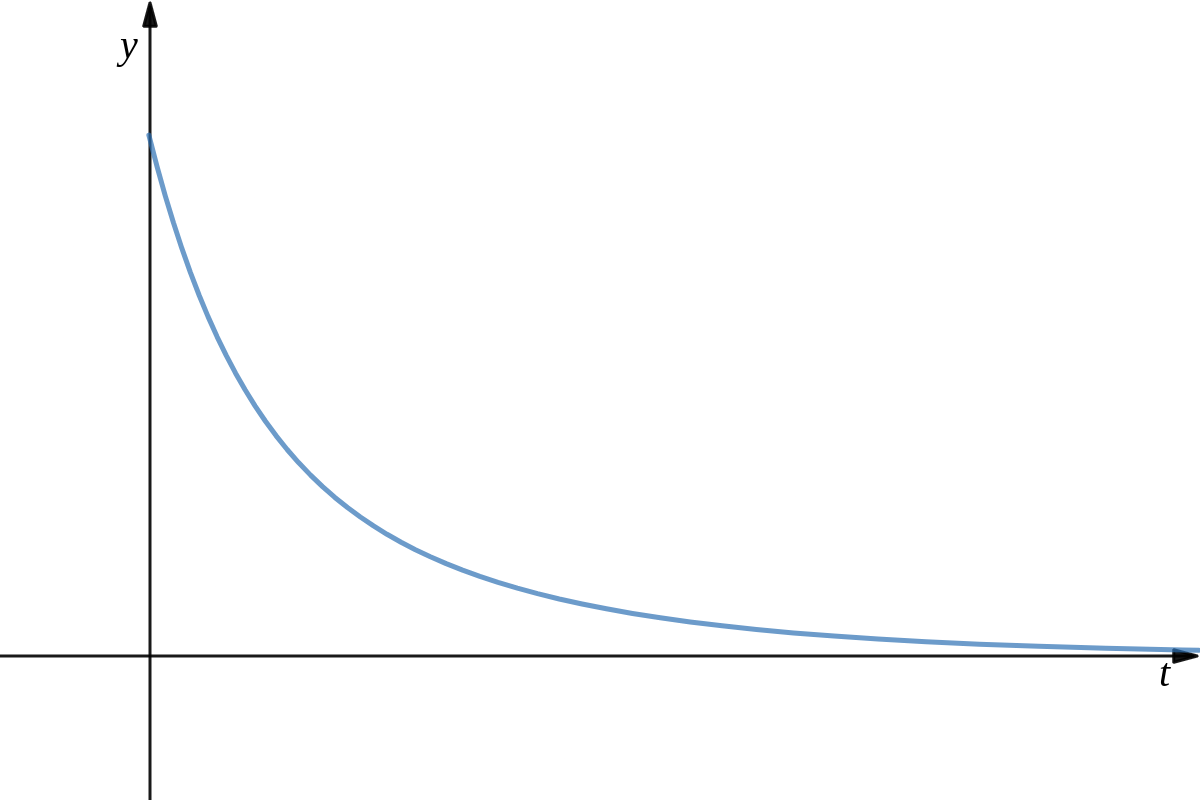
\includegraphics[width=0.69\textwidth]{so9.png}
    \caption{Possible graph of \(x\) vs \(t\).}
\end{figure}
\end{document}
